\chapter{Hiện thực ứng dụng webfuzzer}
Chương này mô tả chi tiết hiện thực của kiến trúc hệ thống ứng dụng webfuzzer, bao gồm ba thành phần backend, \acrshort{ui} và cơ sở dữ liệu của ứng dụng.
\section{Backend}
\subsection{Phần mở rộng Burp Suite}
Phần mở rộng Burp Suite cho phép gửi \acrshort{http} request mẫu từ mô-đun \textbf{Intruder} của Burp Suite đến công cụ \textbf{webfuzzer} theo định dạng JSON như Đoạn mã \ref{lst:base-request-format} dưới đây, quá trình chọn và gửi request mẫu sẽ được trình bày ở \textbf{Phụ lục A} của luận văn.
\begin{lstlisting}[style=ES6, label={lst:base-request-format}, caption={Cấu trúc của một HTTP request mẫu được gửi từ phần mở rộng Burp Suite}]
{
    "python": { 
        "url":"http://testphp.vulnweb.com:80/search.php?test=query",
        "cookies":"",
        "headers":{ 
            "User-Agent":"Mozilla/5.0 (X11; Ubuntu; Linux x86_64; rv:71.0) Gecko/20100101 Firefox/71.0",
            "Accept":"text/html,application/xhtml+xml,application/xml; q=0.9,*/*;q=0.8",
            "Accept-Language":"en-US,en;q=0.5",
            "Accept-Encoding":"gzip, deflate",
            "Content-Type":"application/x-www-form-urlencoded",
            "Origin":"http://testphp.vulnweb.com",
            "DNT":"1",
            "Connection":"close",
            "Referer":"http://testphp.vulnweb.com/search.php?test=query",
            "Upgrade-Insecure-Requests":"1"
        },
        "data":{ 
            "searchFor":"\xa7a\xa7",
            "goButton":"go"
        },
        "method":"post"
    }
}
\end{lstlisting}
Chuỗi ``\texttt{\textbackslash xa7}'' trong trường \texttt{data.searchFor} biểu thị kí tự ``\$'' trong request mẫu. Các kí tự này thường nằm ở trường \texttt{data} hoặc \texttt{url} trong đoạn dữ liệu JSON để đánh dấu những vị trí chèn payload để ứng dụng web xử lí. 
\subsection{Cấu hình kiểm thử}
Điểm chung của những lỗ hổng bảo mật đã giới thiệu ở \textbf{Chương 3} là đều có thể bị khai thác bằng dữ liệu đầu vào từ phía người dùng. Vì thế, ta có thể phát hiện các lỗ hổng này bằng cách thử gửi nhiều dạng payload kiểm thử theo các tham số của \acrshort{http} request và phân tích phản hồi của máy chủ trong response trả về, việc làm này đặc biệt phù hợp với phương pháp fuzzing. Cụ thể giới hạn và phương pháp phát hiện của ứng dụng \textbf{webfuzzer} đối với từng lớp lỗ hổng như sau.
\begin{itemize}
    \item \acrshort{lfi}: ứng dụng tập trung phát hiển lỗ hổng này trên các máy chủ web dùng hệ điều hành nhân Unix. Cụ thể ứng dụng sẽ dùng những payload như Hình \ref{fig:lfi-payloads} để cố gắng đọc nội dung tập tin \texttt{/etc/passwd}. Ứng dụng sẽ kiểm tra \acrshort{http} response trả về xem có xuất hiện chuỗi ``\textbf{root:x}'' hoặc khớp với các biểu thức chính quy hay không để kết luận.
    \item Time-based \acrshort{sqli}: ứng dụng phát hiện tốt trên các ứng dụng web sử dụng các hệ quản trị cơ sở dữ liệu MySQL, Microsoft SQL Server và Postgres SQL bằng cách sử dụng các payload có chứa các hàm hoãn thời gian (đã đề cập ở \textbf{Phần 3.3}) của cả ba hệ quản trị cơ sở dữ liệu này, sau đó căn cứ vào thời gian phản hồi của \acrshort{http} response để kết luận.
\end{itemize}
Các payload, biểu thức chính quy, kĩ thuật tấn công, làm rối sử dụng trong ứng dụng được tổng hợp từ kinh nghiệm của chúng tôi và tổng hợp từ các kho lưu trữ (repository) mã nguồn trên GitHub \parencite{seclist-fuzzing,0verpwn-fuzzing}, từ nhiều blog chia sẻ cũng như write-up các thử thách cướp cờ (capture the flag - CTFs) của đàn anh đi trước trong ngành, từ các tweet được các kĩ sư bảo mật hàng đầu chia sẻ trên mạng xã hội Twitter,... Sau đó các payload này sẽ được chúng tôi chọn lọc và sửa đổi cho phù hợp với phương pháp kiểm thử của ứng dụng như sau.
\begin{itemize}
    \item Đối với các payload time-based \acrshort{sqli}, chúng tôi sử dụng các payload chứa hai loại hàm chính để hoãn thời gian thực hiện request. Cụ thể là hàm \texttt{sleep} (đối với MySQL, tương tự là \texttt{pg\_sleep} đối với PostgreSQL và \texttt{waitfor delay}, \texttt{waitfor time} đối với Microsoft SQL Server) và hàm \\\texttt{BENCHMARK(10000000,MD5('Y4T0G4M11337'))} để kéo dài thời gian thực hiện request đối với các ứng dụng web mắc lỗi này. Bên cạnh đó, với mỗi payload gốc, chúng tôi áp dụng thêm nhiều cách thức đóng ngoặc, chú thích để tránh gặp lỗi cú pháp khi thực thi đoạn mã SQL ở phía máy chủ.
    \item Đối với các payload \acrshort{lfi}, chúng tôi thu thập 8 payload mẫu với số lượng các chuỗi ``../'' tăng dần, nhằm tăng độ sâu của đường dẫn để tiếp cận được tập tin \texttt{/etc/passwd} của máy chủ. Từ 8 payload này, chúng tôi áp dụng các kĩ thuật làm rối riêng biệt để sinh ra 264 payload khác. Các kĩ thuật này bao gồm encode các chuỗi kí tự ``../'', ``..\textbackslash'' và ``..\textbackslash /'' theo các tập kí tự (charset) ít phổ biến như ``\texttt{..\%c0\%af}'', ``\texttt{..\%252f}'', ``\texttt{\%\%32\%65}'', ``\texttt{..\%\%32\%66}'',  ``\texttt{..\%25c1\%259c}'',... để vượt qua một số kĩ thuật lọc và làm sạch dữ liệu ở phía server-side của máy chủ ứng dụng web.
\end{itemize}
Cụ thể cấu hình được áp dụng trong ứng dụng và biểu thức chính quy áp dụng trong trường hợp phát hiện lỗi \acrshort{lfi} được thể hiện ở Đoạn mã \ref{lst:default-fuzz-config} dưới đây.
\begin{lstlisting}[style=ES6, label={lst:default-fuzz-config}, caption={Cấu hình kiểm thử mặc định}]
    let lfiRegex1 = /Warning: include\(|Warning: unlink\(|for inclusion \(include_path=|fread\(|Failed opening required|Warning: file_get_contents\(|Fatal error: require_once\(|Warning: file_exists\(/g;
    let lfiRegex2 = /java\.io\.FileNotFoundException|java\.lang\.Exception|java\.lang\ .IllegalArgumentException|java\.net\.MalformedURLException/g;
    let defaultFuzzConfig = {
        "1": { "label": "Local File Inclusion", "time": "", "match": ["root:x", "localhost"], "payloadFile": "lfi/lfi-full.txt", "matchFile": "", "regex": [lfiRegex1, lfiRegex2] },
        "2": { "label": "Time-based SQL Injection", "time": 10, "match": "", "payloadFile": "sqli/sqli-time-based.txt", "matchFile": "", "regex": [sqliRegex] },
        "3": { "label": "Remote Code Execution", "time": 10, "match": "", "payloadFile": "rce.txt", "matchFile": ["root:x", "371337", "99cebf4d56e5168a1915dd72213db9eb"], "regex": "" }
    }
\end{lstlisting}
Các cấu hình kiểm thử được quản lý bằng id dạng số, được định nghĩa và cung cấp từ phía backend thông qua \acrshort{api} để thống nhất giữa ba thành phần của hệ thống trong quá trình thực thi và lưu trữ. Các cấu hình này thường được chúng tôi sử dụng trong quá trình tìm lỗ hổng bảo mật trên các ứng dụng web bằng Burp Suite, chúng tôi sử dụng lại những cấu hình này cho việc kiểm thử ở ứng dụng webfuzzer để tiện so sánh và đánh giá kết quả hiện thực ứng dụng. Vì gặp khó khăn trong việc truyền biểu thức chính quy trong Node.js qua lại giữa \acrshort{ui} và cơ sở dữ liệu (bao gồm việc chuỗi hóa để lưu vào cơ sở dữ liệu và tái cấu trúc biểu thức chính quy để kiểm thử trên backend) nên hiện tại các cấu hình trên đang được thiết lập trong tập tin \texttt{globalConfig.js} trong thư mục gốc của mã nguồn backend, người dùng có thể sửa đổi các thuộc tính \texttt{payloadFile, match, time,...} trong tập tin trên theo nhu cầu kiểm thử. Ứng dụng chưa hỗ trợ việc thay đổi các thuộc tính này, linh động hóa quá trình thiết lập cấu hình kiểm thử từ phía \acrshort{ui}.\par
\subsection{Thiết lập các biến môi trường}
Các biến môi trường (environment variables) 
\FloatBarrier
\begin{table}[ht]
    \centering
    \caption{Danh sách các biến môi trường ở backend}
    \label{tab:env-variables-backend}
    \begin{tabular}[ht]{ccl}
        \toprule[1pt]\midrule[0.3pt]
            \textbf{Tên biến}&\textbf{Kiểu dữ liệu}&\textbf{Mô tả}\\ 
        \midrule
            SERVICE\_PORT&Integer&Cổng khởi chạy backend của ứng dụng\\
            \addlinespace
            {}&{}&Các thiết lập để kết nối đến dịch vụ MySQL\\
            mysqlConfig&Object&của hệ điều hành, bao gồm host:port, tên\\
            {}&{}&cơ sở dữ liệu và thông tin đăng nhập\\
            \addlinespace
            defaultFuzzConfig&Object&Cấu hình kiểm thử mặc định của ứng dụng\\
            \addlinespace
            defaultVulnTypes&Array&Các lỗ hổng cần kiểm thử đối với trường hợp\\
            {}&{}&tự động tạo yêu cầu kiểm thử\\
            \addlinespace
            fuzzStrategy&String&Chiến thuật kiểm thử mặc định\\
            \addlinespace
            autoCreateFuzzRequest&Boolean&Tự động tạo yêu cầu kiểm thử sau khi nhận \acrshort{http}\\
            {}&{}&request mẫu từ Burp Suite với các lỗ hổng mặc định\\
            \addlinespace
            autoFuzz&Boolean&Tự động thực thi yêu cầu kiểm thử vừa tạo nếu\\
            {}&{}&không có yêu cầu nào khác đang được thực thi\\
            \addlinespace
            autoExecuteQueuedRequest&Boolean&Tự động thực thi một yêu cầu kiểm thử đã tạo\\
            {}&{}&ngay khi thực thi xong yêu cầu hiện tại\\
            \addlinespace
            encodeUrl&Boolean&Encode \acrshort{url} của \acrshort{http} request kiểm thử gửi đi\\
        \midrule[0.3pt]\bottomrule[1pt]
    \end{tabular}
\end{table}
\subsection{Giao diện lập trình ứng dụng - API}
Hình \ref{fig:swagger-api} dưới đây mô tả tổng thể các \acrshort{api} mà backend của ứng dụng webfuzzer cung cấp.
\begin{figure}[H]
  \centering
    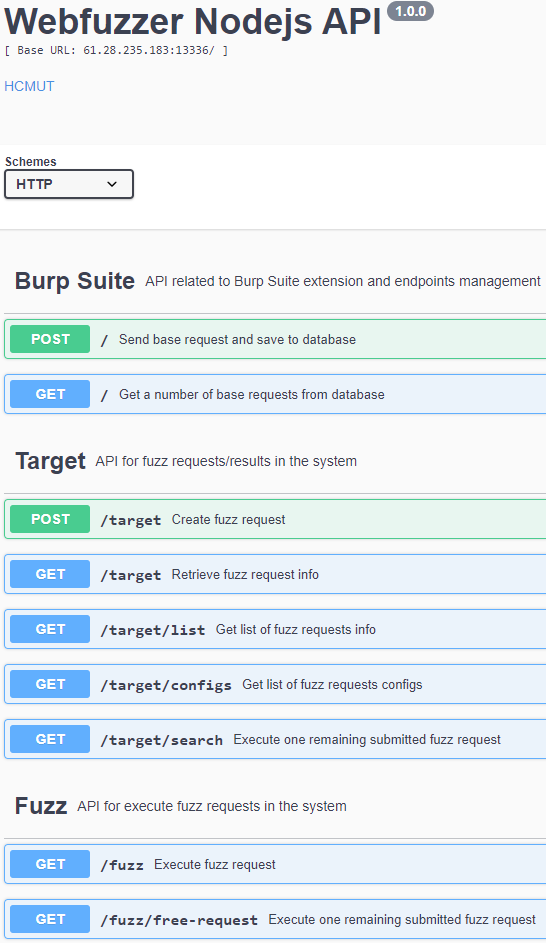
\includegraphics[width=0.5\textwidth,keepaspectratio=true]{images/swagger-api.png}
  \caption{Danh sách các API được cung cấp bởi backend của ứng dụng webfuzzer}
  \label{fig:swagger-api}
\end{figure}
\subsection{Kết nối đến dịch vụ MySQL của hệ điều hành}
\subsection{Mô-đun kiểm thử}
\subsubsection{Mô-đun phân tích request mẫu}
\subsubsection{Mô-đun xây dựng \acrshort{http} request kiểm thử}
\subsubsection{Các mô-đun kiểm thử}
\subsubsection{Mô-đun lưu trữ kết quả kiểm thử}
\section{Giao diện người dùng}
\section{Cơ sở dữ liệu}
Dựa vào thiết kế đã đề ra ở \textbf{Chương 5}, chúng tôi hiện thực cấu trúc cơ sở dữ liệu của ứng dụng webfuzzer gồm ba bảng chính. Bảng \ref{tab:db-tables} dưới đây mô tả tên và chức năng của từng bảng trong lược đồ.
\begin{table}[ht]
    \centering
    \caption{Các bảng trong lược đồ quan hệ}
    \label{tab:db-tables}
    \begin{tabular}[ht]{lll}
        \toprule[1pt]\midrule[0.3pt]
            \textbf{Tên}& &\textbf{Mô tả}\\ 
        \midrule
            Endpoint& &Bảng Endpoint lưu lại các request mẫu mục tiêu được gửi đến máy chủ \\
            {}& &từ phần mở rộng Burp Suite\\
            \addlinespace
            Request& &Bảng Request lưu những yêu cầu kiểm thử một request mẫu \\
            {}& &trong bảng Endpoint của người dùng\\
            \addlinespace
            Result& &Bảng Result lưu kết quả kiểm thử chi tiết \\
            {}& &ứng với mỗi yêu cầu kiểm thử trong bảng Request\\
            \addlinespace
        \midrule[0.3pt]\bottomrule[1pt]
    \end{tabular}
\end{table}
\FloatBarrier
Hình \ref{fig:db-schema} dưới đây mô tả quan hệ giữa các bảng trong lược đồ.
\begin{figure}[H]
  \centering
    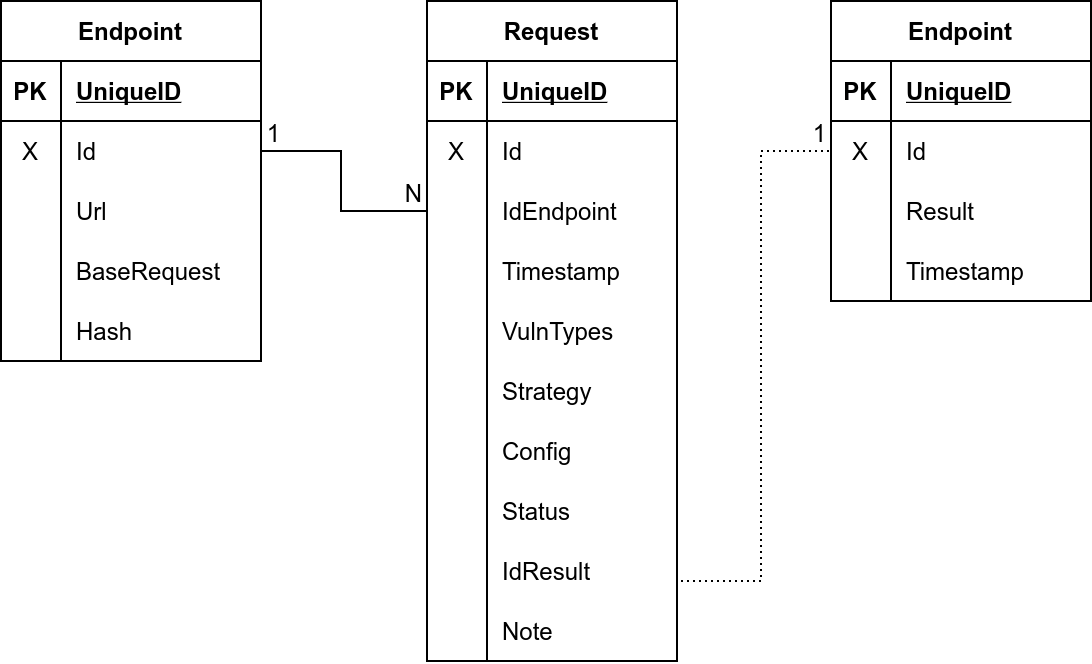
\includegraphics[width=0.75\textwidth,keepaspectratio=true]{images/database-design.png}
  \caption{Sơ đồ mối quan hệ giữa các bảng trong lược đồ}
  \label{fig:db-schema}
\end{figure}
Bảng \texttt{Endpoint} lưu trữ \acrshort{http} request mẫu được gửi từ phần mở rộng Burp Suite đến backend thông qua API \colorbox{gray!30}{\texttt{POST /}}. Request mẫu đó chứa dưới dạng chuỗi dữ liệu JSON trong trường \texttt{BaseRequest}. Trường \texttt{Url} chứa riêng \acrshort{url} của điểm cuối ứng dụng web mục tiêu để thuận lợi trong việc lọc ra những yêu cầu kiểm thử của cùng một trang web thông qua API \colorbox{gray!30}{\texttt{POST /target/search}}. Trường \texttt{Hash} chứa giá trị băm của chuỗi \texttt{BaseRequest}, đảm bảo không lưu hai request mẫu y hệt nhau gây dư thừa dữ liệu. Bảng \texttt{Request} chứa thông tin của các yêu cầu kiểm thử, trong đó trường \texttt{IdEndpoint} là khoá ngoại tham chiếu tới khoá chính \texttt{Id} của bảng \texttt{Endpoint} và trường \texttt{IdResult} là khoá ngoại tham chiếu tới khoá chính \texttt{Id} của bảng \texttt{Result} chứa kết quả kiểm thử (trong trường hợp có lỗ hổng). Mỗi bản ghi trong bảng \texttt{Request} chứa \acrshort{http} request mẫu gửi đến các điểm cuối của ứng dụng web mục tiêu, tập các lỗ hổng cần kiểm thử, trạng thái, và kết quả kiểm thử tương ứng, bao gồm danh sách lỗ hổng của điểm cuối đó và các payload phát hiện được. Trường \texttt{BaseRequest} của bảng \texttt{Endpoint}, trường \texttt{VulnTypes} của bảng \texttt{Request} và \texttt{Result} của bảng \texttt{Result} là các trường có kiểu chuỗi, chứa các giá trị kiểu đối tượng JSON đã được chuỗi hóa như đã đề cập trong phần thiết kế kiến trúc cơ sở dữ liệu ở trên.